\documentclass[11pt,a4paper]{article}
\usepackage[margin=1in]{geometry}
\usepackage{booktabs}
\usepackage{longtable}
\usepackage{graphicx}
\usepackage{xcolor}
\usepackage{tikz}
\usepackage{enumitem}
\usepackage{hyperref}
\usepackage{fancyhdr}
\usepackage{listings}
\usepackage{tcolorbox}

\usetikzlibrary{shapes.geometric, arrows.meta, positioning, calc, patterns}

\pagestyle{fancy}
\fancyhf{}
\rhead{Project Planning Document}
\lhead{Simulation Platform}
\rfoot{Page \thepage}

\definecolor{codegreen}{rgb}{0,0.6,0}
\definecolor{codegray}{rgb}{0.5,0.5,0.5}
\definecolor{codepurple}{rgb}{0.58,0,0.82}
\definecolor{backcolour}{rgb}{0.95,0.95,0.92}

\lstdefinestyle{mystyle}{
    backgroundcolor=\color{backcolour},   
    commentstyle=\color{codegreen},
    keywordstyle=\color{magenta},
    numberstyle=\tiny\color{codegray},
    stringstyle=\color{codepurple},
    basicstyle=\ttfamily\footnotesize,
    breakatwhitespace=false,         
    breaklines=true,                 
    captionpos=b,                    
    keepspaces=true,                 
    numbers=left,                    
    numbersep=5pt,                  
    showspaces=false,                
    showstringspaces=false,
    showtabs=false,                  
    tabsize=2
}
\lstset{style=mystyle}

\newtcolorbox{decision}{
    colback=green!5!white,
    colframe=green!75!black,
    title=Key Decision
}

\newtcolorbox{warning}{
    colback=red!5!white,
    colframe=red!75!black,
    title=Warning
}

\newtcolorbox{insight}{
    colback=blue!5!white,
    colframe=blue!75!black,
    title=Insight
}

\title{Simulation Platform Project Plan\\[0.5em]\large From Layout Editor to Heavy Manufacturing Simulation\\[0.5em]\small Comprehensive Planning Dialog}
\author{Technical Reference Document}
\date{\today}

\begin{document}

\maketitle

\begin{abstract}
This document captures the complete planning dialog for a simulation platform targeting factory and heavy manufacturing (shipbuilding) applications. It records the evolution from a 2D layout editor concept through to a tiered architecture integrating WPF, Unity, and discrete event simulation. Key decisions, rejected approaches, and the final architecture are documented for ongoing reference.
\end{abstract}

\tableofcontents
\newpage

%==============================================================================
\section{Project Genesis: The Layout Editor}
%==============================================================================

The project began as a layout editor for discrete event simulation, with an initial focus on transport layer management.

\subsection{Initial Transport Layer Concept}

The original concept proposed a layered approach to transportation definition:

\begin{enumerate}
    \item Lay down building walls and zones
    \item Place machines
    \item Define cells and local flows (no transporters required)
    \item Define AGV and EOT crane routes (constrained layer)
    \item Define forklift and pallet jack routes (less constrained layer)
    \item Overlay pedestrian mesh with unsafe zones removed
\end{enumerate}

\subsection{Refined Layer Architecture}

After review, the layer hierarchy was refined:

\begin{table}[h]
\centering
\caption{Transport Layer Hierarchy (Revised)}
\begin{tabular}{@{}cllp{5cm}@{}}
\toprule
\textbf{Layer} & \textbf{Name} & \textbf{Constraint} & \textbf{Contents} \\
\midrule
0 & Fixed Infrastructure & Immutable & Building, columns, crane runways, doors \\
1 & Spatial Planning & Semi-fixed & Zones, primary aisles, restricted areas \\
2 & Equipment & Placed & Machines, buffers, workstations \\
3 & Local Flow & Connected & Cells, direct paths, conveyors \\
4 & Guided Transport & Track-bound & AGV paths, stations, traffic zones \\
5 & Overhead Transport & Runway-bound & EOT cranes, jib cranes, coverage \\
6 & Flexible Transport & Aisle-constrained & Forklift aisles, staging areas \\
7 & Pedestrian & Mesh-based & Walkable polygons, crossings \\
\bottomrule
\end{tabular}
\end{table}

\begin{decision}
\textbf{Crane runways at Layer 0}: Crane infrastructure is structural, installed with the building. It constrains machine layout, not vice versa.
\end{decision}

\begin{decision}
\textbf{Primary aisles at Layer 1}: Define pedestrian routes early, not as ``what's left over.'' Safety regulations mandate specific routes.
\end{decision}

%==============================================================================
\section{Critical Assessment: Layout vs. Simulation}
%==============================================================================

\begin{warning}
The initial architecture was a \textbf{layout editor architecture}, not a \textbf{simulator architecture}. It answered ``where are things located'' but not ``what happens over time.''
\end{warning}

\subsection{Identified Gaps}

\begin{table}[h]
\centering
\caption{Missing Simulation Components}
\begin{tabular}{@{}ll@{}}
\toprule
\textbf{Gap} & \textbf{What's Missing} \\
\midrule
Time model & Discrete event scheduler, clock, run control \\
Entity model & Parts, loads, jobs, orders — things that flow \\
Behavior specification & Decision logic for AGVs, cranes, workers \\
Performance parameters & Process times, speeds, breakdown rates \\
Stochastic elements & Distributions, random variability \\
\bottomrule
\end{tabular}
\end{table}

\subsection{The NavMesh Misconception}

\begin{warning}
Triangulated navigation meshes are for real-time games with continuous pathfinding. Discrete event simulation uses distance/time matrices between discrete nodes. The pedestrian mesh was solving the wrong problem for DES.
\end{warning}

%==============================================================================
\section{Tiered Architecture Decision}
%==============================================================================

\subsection{The Three-Tier Model}

\begin{decision}
Separate the system into three tiers, each with distinct responsibilities:
\begin{enumerate}
    \item \textbf{Layout Tier}: Static geometry, equipment placement, transport infrastructure
    \item \textbf{Parts Tier}: Process logic, routing, material flow definitions
    \item \textbf{Simulation Tier}: Time progression, events, resource contention, statistics
\end{enumerate}
All tiers read and write to a shared database.
\end{decision}

\begin{figure}[h]
\centering
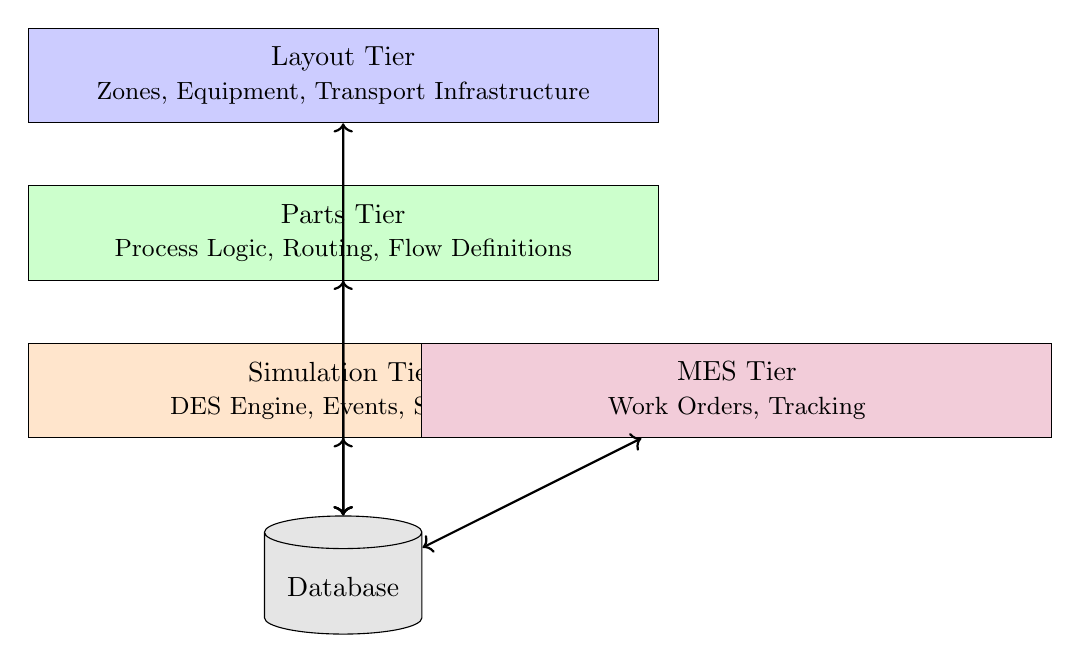
\begin{tikzpicture}[
    tier/.style={rectangle, draw, minimum width=8cm, minimum height=1.2cm, align=center},
    db/.style={cylinder, draw, shape border rotate=90, aspect=0.25, minimum height=1.5cm, minimum width=2cm},
    arrow/.style={-{Stealth}, thick}
]
    \node[tier, fill=blue!20] (layout) at (0,4) {Layout Tier\\{\small Zones, Equipment, Transport Infrastructure}};
    \node[tier, fill=green!20] (parts) at (0,2) {Parts Tier\\{\small Process Logic, Routing, Flow Definitions}};
    \node[tier, fill=orange!20] (sim) at (0,0) {Simulation Tier\\{\small DES Engine, Events, Statistics}};
    \node[tier, fill=purple!20] (mes) at (5,0) {MES Tier\\{\small Work Orders, Tracking}};
    
    \node[db, fill=gray!20] (db) at (0,-2.5) {Database};
    
    \draw[arrow, <->] (layout) -- (db);
    \draw[arrow, <->] (parts) -- (db);
    \draw[arrow, <->] (sim) -- (db);
    \draw[arrow, <->] (mes) -- (db);
\end{tikzpicture}
\caption{Tiered architecture with shared database}
\end{figure}

\subsection{Database as Integration Layer}

\begin{decision}
\textbf{SQLite as source of truth.} PostgreSQL for team/deployed scenarios, JSON for debugging. SQLite is the canonical format --- portable, versionable, single file.
\end{decision}

\begin{insight}
Database as integration layer allows:
\begin{itemize}
    \item Swapping simulation engines without rewriting layout tools
    \item Running different tools against the same layout
    \item MES integration via standard database queries
    \item Independent development and testing of tiers
\end{itemize}
\end{insight}

\subsection{Derived Data Responsibility}

\begin{table}[h]
\centering
\caption{Data Computation Options}
\begin{tabular}{@{}lp{8cm}@{}}
\toprule
\textbf{Option} & \textbf{Trade-off} \\
\midrule
Layout exports raw, simulation computes & Clean but duplicated computation \\
Layout pre-computes paths to DB & Efficient but layout needs speed parameters \\
Middleware service on demand & Adds component complexity \\
\bottomrule
\end{tabular}
\end{table}

%==============================================================================
\section{The 3D Question}
%==============================================================================

\subsection{Initial Assessment}

For standard factory simulation, 3D is largely cosmetic:
\begin{itemize}
    \item Layout is fundamentally 2D + height
    \item 3D models are visual decoration attached to nodes
    \item Collision and routing use simplified bounding geometry
    \item No major simulation tool pathfinds through B-rep surfaces
\end{itemize}

\subsection{Heavy Manufacturing Changes Everything}

\begin{insight}
In shipbuilding, aerospace, and heavy equipment manufacturing:
\begin{itemize}
    \item The \textbf{product is the environment} --- workers move through it
    \item Assembly sequence determines accessibility
    \item Layout \textbf{evolves} as the product is built
    \item Planning question: ``Can we do operation X before installing component Y?''
\end{itemize}
\end{insight}

\begin{table}[h]
\centering
\caption{Standard Factory vs. Heavy Manufacturing}
\begin{tabular}{@{}ll@{}}
\toprule
\textbf{Standard Factory} & \textbf{Heavy Manufacturing} \\
\midrule
Product is a token & Product is geometry \\
Product moves through space & Workers move through product \\
Layout is static & Layout evolves during build \\
2D + height sufficient & True 3D required \\
Pathfinding on floor & Pathfinding on surfaces, scaffolds \\
Equipment has footprint & Equipment has reach envelope \\
\bottomrule
\end{tabular}
\end{table}

\subsection{Target Market Confirmation}

\begin{decision}
Target market includes shipbuilding and heavy manufacturing. This requires Unity integration and 3D product geometry. The shipyard contact exists --- this is a real project, not speculation.
\end{decision}

%==============================================================================
\section{Revised Architecture: WPF + Unity + Simulation}
%==============================================================================

\subsection{Component Responsibilities}

\begin{figure}[h]
\centering
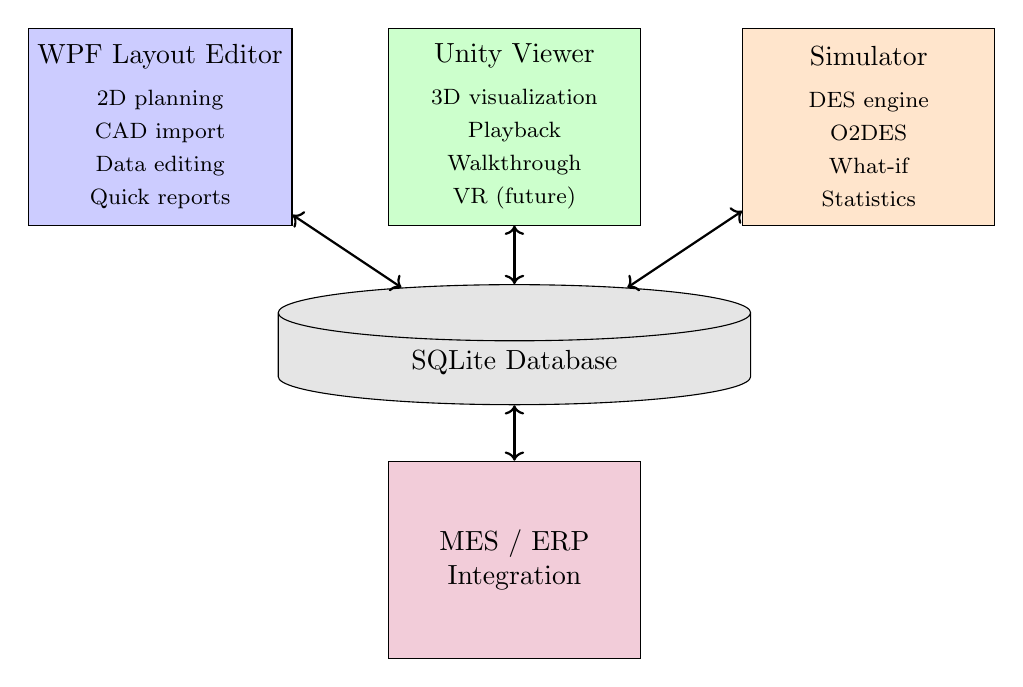
\begin{tikzpicture}[
    comp/.style={rectangle, draw, minimum width=3.2cm, minimum height=2.5cm, align=center},
    db/.style={cylinder, draw, shape border rotate=90, aspect=0.25, minimum height=1cm, minimum width=6cm},
    arrow/.style={-{Stealth}, thick}
]
    \node[db, fill=gray!20] (db) at (0,0) {SQLite Database};
    
    \node[comp, fill=blue!20] (wpf) at (-4.5,3) {WPF Layout Editor\\[0.3em]{\footnotesize 2D planning}\\{\footnotesize CAD import}\\{\footnotesize Data editing}\\{\footnotesize Quick reports}};
    
    \node[comp, fill=green!20] (unity) at (0,3) {Unity Viewer\\[0.3em]{\footnotesize 3D visualization}\\{\footnotesize Playback}\\{\footnotesize Walkthrough}\\{\footnotesize VR (future)}};
    
    \node[comp, fill=orange!20] (sim) at (4.5,3) {Simulator\\[0.3em]{\footnotesize DES engine}\\{\footnotesize O2DES}\\{\footnotesize What-if}\\{\footnotesize Statistics}};
    
    \node[comp, fill=purple!20] (mes) at (0,-2.5) {MES / ERP\\Integration};
    
    \draw[arrow, <->] (wpf) -- (db);
    \draw[arrow, <->] (unity) -- (db);
    \draw[arrow, <->] (sim) -- (db);
    \draw[arrow, <->] (mes) -- (db);
\end{tikzpicture}
\caption{Final architecture: Three applications, shared database}
\end{figure}

\begin{decision}
\textbf{WPF and Unity are separate applications}, not embedded. Both read/write the same database. User switches between apps as needed. This is simpler, more maintainable, and leverages each platform's strengths.
\end{decision}

\subsection{What Each Component Does}

\textbf{WPF Layout Editor:}
\begin{itemize}
    \item 2D floor plan editing
    \item Zone and equipment placement
    \item Transport path definition
    \item CAD import (DXF priority)
    \item Database editing interface
    \item Quick 2D visualization
\end{itemize}

\textbf{Unity Viewer:}
\begin{itemize}
    \item 3D visualization of facility and products
    \item Playback of simulation results (like a video player)
    \item Walkthrough for planning review
    \item Visual validation of access constraints
    \item Client presentations
    \item Future: VR support (built into Unity)
\end{itemize}

\textbf{Simulator (O2DES):}
\begin{itemize}
    \item Discrete event simulation engine
    \item Reads layout and process definitions from DB
    \item Executes with stochastic variability
    \item Writes timestamped events to DB
    \item No graphics --- pure computation
\end{itemize}

\begin{warning}
\textbf{Unity does NOT:}
\begin{itemize}
    \item Run the simulation
    \item Make scheduling decisions
    \item Compute task times
    \item Resolve resource conflicts
\end{itemize}
Unity is a 3D video player for simulation results.
\end{warning}

%==============================================================================
\section{The 2D/3D Unification}
%==============================================================================

\subsection{Core Insight}

\begin{insight}
The simulation engine doesn't care about dimensions. Events are geometry-agnostic:
\begin{verbatim}
Event: AGV_123 arrives at Station_A
Event: Worker_7 starts Operation_45
Event: Crane_2 picks Load_89
\end{verbatim}
These are identical whether visualized in 2D or 3D.
\end{insight}

\subsection{Configuration, Not Code Branching}

\begin{lstlisting}[language=C, caption=Layout configuration model]
LayoutSettings
{
    SimulationType: "2D" | "3D" | "Hybrid"
    ProductGeometry: null | PathToCAD
    WorkerModel: "Simple" | "Posture" | "FullErgonomic"
    Visualization: "WPF" | "Unity" | "Both"
}
\end{lstlisting}

\begin{table}[h]
\centering
\caption{Configuration by Use Case}
\begin{tabular}{@{}llll@{}}
\toprule
\textbf{Setting} & \textbf{2D Factory} & \textbf{Shipyard} \\
\midrule
ProductGeometry & null & Path to STEP/glTF \\
WorkerModel & Simple & Posture \\
Visualization & WPF & Unity \\
\bottomrule
\end{tabular}
\end{table}

\begin{decision}
One product with a capability dial. Turn left: 2D factory simulation. Turn right: 3D shipyard planning with VR walkthrough. Same architecture, scalable complexity.
\end{decision}

\subsection{Access Points as Resources}

\begin{warning}
\textbf{Critical requirement:} Access constraints must be enforced in the simulation, not just visualized in Unity. Otherwise, schedules will be produced that cannot execute.
\end{warning}

\begin{lstlisting}[language=SQL, caption=Access as resource constraint]
-- Access points become resources in scheduling
Operation A requires AccessPoint_7
Operation B requires AccessPoint_7
-- Simulation must sequence them, not overlap them
\end{lstlisting}

Access points are resources like workers and cranes. The scheduling engine handles contention. Unity shows the result.

%==============================================================================
\section{Feasibility Assessment}
%==============================================================================

\subsection{Team Reality}

\begin{itemize}
    \item One principal developer
    \item Possibly 2 students (net cost for 3-6 months, productive for 6-12 months, then leave)
\end{itemize}

\textbf{Students suitable for:}
\begin{itemize}
    \item Defined, isolated modules
    \item Testing
    \item Documentation
    \item UI polish
\end{itemize}

\textbf{Students NOT suitable for:}
\begin{itemize}
    \item Core architecture
    \item Simulation engine
    \item Anything on critical path
\end{itemize}

\subsection{Build vs. Integrate}

\begin{table}[h]
\centering
\caption{Component Strategy}
\begin{tabular}{@{}lccc@{}}
\toprule
\textbf{Component} & \textbf{Build} & \textbf{Integrate} & \textbf{Complexity} \\
\midrule
WPF layout editor & \checkmark & & Medium (mostly done) \\
Database schema & \checkmark & & Low \\
DES core & & \checkmark (O2DES) & Low \\
Scheduling engine & & \checkmark (existing) & Don't build \\
Unity viewer & \checkmark & & Medium \\
VR support & & \checkmark (Unity built-in) & Low \\
CAD import & & \checkmark (libraries) & Low-Medium \\
\bottomrule
\end{tabular}
\end{table}

\begin{decision}
\textbf{O2DES for simulation engine.} Lightweight, C\#, open source. Runs in days, not weeks. Don't build custom DES --- it's solved.
\end{decision}

\begin{decision}
\textbf{Existing scheduler.} Multi-person, multi-resource scheduling is hard and solved. Use what exists.
\end{decision}

\subsection{What NOT to Build}

\begin{warning}
Do not attempt to compete with Aveva, Dassault, Siemens on features. They have 200+ person teams and 20+ year head starts.
\end{warning}

The viable path is solving a specific problem for a specific customer, not building a general platform.

%==============================================================================
\section{The Final Plan}
%==============================================================================

\subsection{Parallel Development Tracks}

\begin{decision}
Develop three tracks in parallel, integrate later:
\begin{itemize}
    \item \textbf{Track A:} WPF Layout $\rightarrow$ SQLite $\rightarrow$ O2DES simulation
    \item \textbf{Track B:} Unity factory walkthrough (standalone)
    \item \textbf{Track C:} Integration (simulation feeds Unity)
\end{itemize}
Track A and B can demo independently. Track C only matters once both work.
\end{decision}

\begin{figure}[h]
\centering
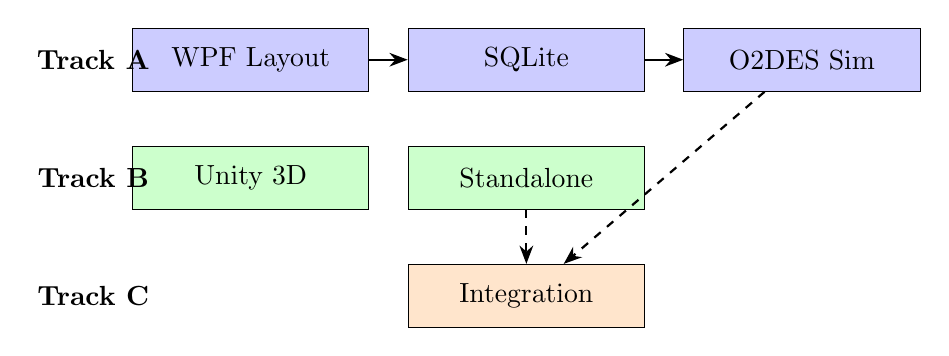
\begin{tikzpicture}[
    track/.style={rectangle, draw, minimum width=3cm, minimum height=0.8cm, align=center},
    arrow/.style={-{Stealth}, thick}
]
    \node[track, fill=blue!20] (a1) at (0,2) {WPF Layout};
    \node[track, fill=blue!20] (a2) at (3.5,2) {SQLite};
    \node[track, fill=blue!20] (a3) at (7,2) {O2DES Sim};
    \node at (-2,2) {\textbf{Track A}};
    
    \node[track, fill=green!20] (b1) at (0,0.5) {Unity 3D};
    \node[track, fill=green!20] (b2) at (3.5,0.5) {Standalone};
    \node at (-2,0.5) {\textbf{Track B}};
    
    \node[track, fill=orange!20] (c1) at (3.5,-1) {Integration};
    \node at (-2,-1) {\textbf{Track C}};
    
    \draw[arrow] (a1) -- (a2);
    \draw[arrow] (a2) -- (a3);
    \draw[arrow, dashed] (a3) -- (c1);
    \draw[arrow, dashed] (b2) -- (c1);
\end{tikzpicture}
\caption{Parallel development tracks}
\end{figure}

\subsection{Event Schema: Define First}

\begin{decision}
Define the timestamped event schema before building simulation or Unity viewer. Both will read/write it.
\end{decision}

\begin{lstlisting}[language=SQL, caption=Simulation event schema]
CREATE TABLE sim_events (
    id INTEGER PRIMARY KEY,
    sim_time REAL,              -- simulation clock
    wall_time TEXT,             -- when event was written
    entity_type TEXT,           -- 'Part', 'Worker', 'Crane', etc.
    entity_id TEXT,
    event_type TEXT,            -- 'Arrive', 'StartOp', 'EndOp', 'Move'
    location_id TEXT,
    data TEXT                   -- JSON blob for extras
);

CREATE INDEX idx_sim_time ON sim_events(sim_time);
CREATE INDEX idx_entity ON sim_events(entity_id);
\end{lstlisting}

Unity queries by \texttt{sim\_time} range, animates entities to locations. Simple, decoupled, debuggable.

\subsection{Integration Model}

\begin{lstlisting}[caption=Data flow]
Simulation runs
    |
    v
Writes timestamped events to SQLite
    |
    v
Unity reads events by time range
    |
    v
Animates: entities appear at locations
          buffers fill/empty
          workers move to stations
\end{lstlisting}

\begin{insight}
\textbf{Buffer visualization is high value, low complexity.} Crowded input bays, empty buffers, WIP accumulation --- visible at a glance. Executives understand a picture of a clogged factory floor. This sells the tool.
\end{insight}

\subsection{Timeline}

\begin{table}[h]
\centering
\caption{Development Timeline}
\begin{tabular}{@{}clp{7cm}@{}}
\toprule
\textbf{Phase} & \textbf{Duration} & \textbf{Deliverable} \\
\midrule
1 & 2 months & Finish WPF editor, solidify DB schema \\
2 & 2 months & O2DES integration, schedule import, event logging \\
3 & 2 months & Unity viewer, playback, buffer visualization \\
4 & 1 month & Integration, pilot with shipyard \\
5 & Ongoing & Iterate based on feedback \\
\midrule
& \textbf{7-8 months} & \textbf{Pilot-ready} \\
\bottomrule
\end{tabular}
\end{table}

%==============================================================================
\section{Risk Management}
%==============================================================================

\begin{table}[h]
\centering
\caption{Key Risks and Mitigations}
\begin{tabular}{@{}p{4cm}p{8cm}@{}}
\toprule
\textbf{Risk} & \textbf{Mitigation} \\
\midrule
Schema mismatch between projects & Define shared schema in one place; both projects reference it \\
Unity polling DB is slow & Batch reads; or simulation writes to file Unity watches \\
Time sync confusion & Strict convention: Unity only uses sim\_time for playback \\
Scope creep & Pilot with one customer first; expand based on revenue \\
Student turnover & Keep students off critical path; document everything \\
\bottomrule
\end{tabular}
\end{table}

%==============================================================================
\section{Customer Engagement}
%==============================================================================

\subsection{Essential Questions for Shipyard Meeting}

\begin{enumerate}
    \item What planning decision costs you the most when you get it wrong?
    \item What tools do you use now? What's broken about them?
    \item Show me how you plan block assembly sequence today.
    \item When did you last have a crane wait because access wasn't ready?
    \item When did you last re-work because something was installed out of sequence?
    \item What would you pay to fix that?
\end{enumerate}

\begin{decision}
\textbf{Don't pitch software. Listen.} Look for the expensive pain point, not confirmation of your vision.
\end{decision}

\subsection{Required from Customer}

\begin{itemize}
    \item Sample data: block model, work package list, schedule extract
    \item Access to planners who do this work daily
    \item Willingness to pilot (ideally with some funding or guaranteed purchase)
\end{itemize}

%==============================================================================
\section{Technical Specifications}
%==============================================================================

\subsection{Layer Model (Facility)}

\begin{lstlisting}[language=SQL, caption=Core facility tables]
CREATE TABLE zones (
    id TEXT PRIMARY KEY,
    name TEXT,
    category TEXT,
    x REAL, y REAL, width REAL, height REAL,
    fill_color TEXT,
    floor TEXT
);

CREATE TABLE equipment (
    id TEXT PRIMARY KEY,
    name TEXT,
    type TEXT,
    x REAL, y REAL, width REAL, depth REAL,
    height REAL DEFAULT NULL,           -- 3D extension
    model_path TEXT DEFAULT NULL,       -- 3D extension
    zone_id TEXT REFERENCES zones(id)
);

CREATE TABLE transport_paths (
    id TEXT PRIMARY KEY,
    path_type TEXT,                     -- 'AGV', 'Forklift', 'Crane'
    layer INTEGER,
    geometry TEXT                       -- JSON polyline
);
\end{lstlisting}

\subsection{Product Model (Heavy Manufacturing)}

\begin{lstlisting}[language=SQL, caption=Product/assembly tables]
CREATE TABLE product_components (
    id TEXT PRIMARY KEY,
    name TEXT,
    parent_id TEXT REFERENCES product_components(id),
    geometry_path TEXT,                 -- Path to STEP/glTF
    installation_state TEXT             -- 'Planned', 'InProgress', 'Complete'
);

CREATE TABLE operations (
    id TEXT PRIMARY KEY,
    name TEXT,
    component_id TEXT REFERENCES product_components(id),
    duration_mean REAL,
    duration_stddev REAL,
    required_resources TEXT,            -- JSON array
    required_access_points TEXT         -- JSON array
);

CREATE TABLE precedence (
    predecessor_id TEXT REFERENCES operations(id),
    successor_id TEXT REFERENCES operations(id),
    PRIMARY KEY (predecessor_id, successor_id)
);

CREATE TABLE access_points (
    id TEXT PRIMARY KEY,
    name TEXT,
    x REAL, y REAL, z REAL,
    capacity INTEGER DEFAULT 1          -- How many workers can use simultaneously
);
\end{lstlisting}

\subsection{Simulation Events}

\begin{lstlisting}[language=SQL, caption=Event log for Unity playback]
CREATE TABLE sim_events (
    id INTEGER PRIMARY KEY AUTOINCREMENT,
    sim_time REAL NOT NULL,
    wall_time TEXT NOT NULL,
    entity_type TEXT NOT NULL,
    entity_id TEXT NOT NULL,
    event_type TEXT NOT NULL,
    location_id TEXT,
    data TEXT
);

CREATE INDEX idx_events_time ON sim_events(sim_time);
CREATE INDEX idx_events_entity ON sim_events(entity_type, entity_id);

-- Example events:
-- (1, 0.0, '2024-01-15T10:00:00', 'Worker', 'W1', 'StartOp', 'OP_45', '{"tool":"welder"}')
-- (2, 2.5, '2024-01-15T10:00:01', 'Worker', 'W1', 'EndOp', 'OP_45', '{}')
-- (3, 2.5, '2024-01-15T10:00:01', 'Part', 'P100', 'Move', 'Buffer_3', '{}')
\end{lstlisting}

\subsection{Buffer State for Visualization}

\begin{lstlisting}[language=SQL, caption=Buffer state snapshots]
CREATE TABLE buffer_states (
    id INTEGER PRIMARY KEY AUTOINCREMENT,
    sim_time REAL NOT NULL,
    buffer_id TEXT NOT NULL,
    quantity INTEGER NOT NULL,
    contents TEXT                       -- JSON array of part IDs
);

CREATE INDEX idx_buffer_time ON buffer_states(sim_time);
\end{lstlisting}

%==============================================================================
\section{Opening Model}
%==============================================================================

Openings are edges in the movement graph connecting zones. All openings share a common model; doors, hatches, and aisles are instances with different default properties.

\subsection{Core Abstraction}

Every passage between zones is an opening. The key insight: capacity = 0 means unconstrained (no token required), but the opening still has state and can be closed.

\begin{table}[h]
\centering
\caption{Capacity Semantics}
\begin{tabular}{@{}lll@{}}
\toprule
\textbf{Capacity} & \textbf{Behavior} & \textbf{Example} \\
\midrule
0 & Check state only, no token & Wide aisle, bay entrance \\
1 & Acquire token, one at a time & Personnel door, manhole \\
N & Acquire token, up to N simultaneous & Dock door, scaffold access \\
\bottomrule
\end{tabular}
\end{table}

\begin{decision}
\textbf{Doors are openings}: A door is an opening with capacity $\geq$ 1 plus door-specific properties (swing, access control). An aisle is an opening with capacity = 0. Both use the same state machine.
\end{decision}

\subsection{Opening Hierarchy}

\begin{lstlisting}[caption=Opening class hierarchy]
Opening (base)
+-- Id, Name, Location (X, Y)
+-- Capacity: 0 = unconstrained, N = token-limited
+-- State: Open | Closed | Locked | Emergency
+-- Dimensions: ClearWidth, ClearHeight, MaxLoadWeight
+-- AllowedEntityTypes: [Worker, Forklift, Pallet, AGV]
+-- DirectionMode: Bidirectional | InboundOnly | OutboundOnly
+-- TraversalTime (seconds, distribution)
+-- Connections: FromZoneId, ToZoneId
+-- BlockingConditions: ["CraneInZone", "FireAlarm"]
|
+-- UnconstrainedOpening (capacity = 0)
|   +-- Aisle (wide corridor)
|   +-- BayEntrance (open area, can be cordoned)
|   +-- EmergencyExit (always capacity 0, special state rules)
|
+-- ConstrainedOpening (capacity >= 1)
|   +-- Door
|   |   +-- SwingDirection, AutoClose, AccessControl
|   +-- Hatch
|   |   +-- IsVertical, LadderTime
|   +-- Manhole
|   |   +-- ConfinedSpaceProtocol, RequiresPermit
|   +-- Airlock
|   |   +-- InnerDoorId, OuterDoorId, CycleTime
|   +-- Gate
|       +-- VehicleOnly, BarrierType
|
+-- TemporaryOpening
    +-- ExistsFromState, ExistsUntilState
    +-- CreatedByOperationId
\end{lstlisting}

\subsection{State Machine}

All openings share the same state machine, regardless of capacity:

\begin{figure}[h]
\centering
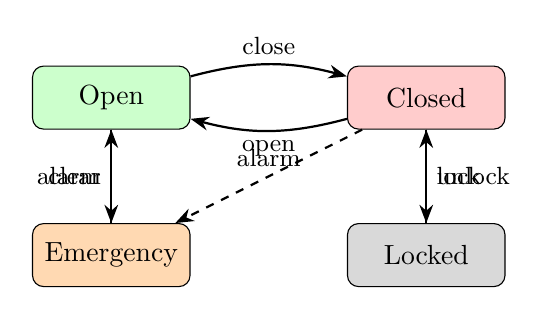
\begin{tikzpicture}[
    state/.style={rectangle, draw, rounded corners, minimum width=2cm, minimum height=0.8cm},
    arrow/.style={-{Stealth}, thick}
]
    \node[state, fill=green!20] (open) at (0,0) {Open};
    \node[state, fill=red!20] (closed) at (4,0) {Closed};
    \node[state, fill=gray!30] (locked) at (4,-2) {Locked};
    \node[state, fill=orange!30] (emergency) at (0,-2) {Emergency};
    
    \draw[arrow, bend left=15] (open) to node[above]{\small close} (closed);
    \draw[arrow, bend left=15] (closed) to node[below]{\small open} (open);
    \draw[arrow] (closed) to node[right]{\small lock} (locked);
    \draw[arrow] (locked) to node[right]{\small unlock} (closed);
    \draw[arrow] (open) to node[left]{\small alarm} (emergency);
    \draw[arrow] (emergency) to node[left]{\small clear} (open);
    \draw[arrow, dashed] (closed) to node[above]{\small alarm} (emergency);
\end{tikzpicture}
\caption{Opening state machine (applies to all opening types)}
\end{figure}

\subsection{Simulation Behavior}

\begin{enumerate}
    \item Entity requests passage through opening
    \item Check state: if not Open, block or reroute
    \item Check entity type against AllowedEntityTypes
    \item Check entity dimensions against ClearWidth/ClearHeight
    \item If capacity = 0: proceed (no token needed)
    \item If capacity $>$ 0: acquire token (block if unavailable)
    \item Delay by TraversalTime
    \item If capacity $>$ 0: release token
\end{enumerate}

\begin{insight}
Unconstrained openings (capacity = 0) still participate in the model. A wide aisle can be closed for crane operations, blocked during emergency, or monitored for traffic statistics --- all without token management overhead.
\end{insight}

\subsection{Why Unconstrained Openings Matter}

\begin{itemize}
    \item \textbf{Emergency scenarios}: Fire alarm $\rightarrow$ close all openings except emergency exits
    \item \textbf{Crane operations}: Overhead lift $\rightarrow$ close all openings in drop zone
    \item \textbf{Shift changes}: After hours $\rightarrow$ lock personnel doors, keep vehicle gates open
    \item \textbf{Traffic analysis}: Track flow through ``unconstrained'' aisles to find hidden bottlenecks
\end{itemize}

\subsection{Opening Types in Shipbuilding}

\begin{table}[h]
\centering
\caption{Opening Instances by Type}
\begin{tabular}{@{}lclp{4.5cm}@{}}
\toprule
\textbf{Type} & \textbf{Capacity} & \textbf{Base Class} & \textbf{Special Properties} \\
\midrule
Wide aisle & 0 & Unconstrained & Can be cordoned \\
Bay entrance & 0 & Unconstrained & Crane interlock \\
Personnel door & 1 & Door & Badge access, swing \\
Watertight door & 1--2 & Door & Dogging mechanism \\
Deck hatch & 1 & Hatch & Ladder time, vertical \\
Manhole & 1 & Manhole & Confined space permit \\
Scaffold access & 2--3 & Constrained & Load limit \\
Temporary cut & 1--2 & Temporary & Assembly state bounds \\
Airlock & 1 & Airlock & Dual door, cycle time \\
\bottomrule
\end{tabular}
\end{table}

\subsection{Database Schema}

\begin{lstlisting}[language=SQL, caption=Opening tables]
CREATE TABLE openings (
    id TEXT PRIMARY KEY,
    name TEXT,
    opening_type TEXT,           -- Aisle, Door, Hatch, Manhole, Airlock, Gate
    x REAL,
    y REAL,
    
    -- Capacity (0 = unconstrained)
    capacity INTEGER DEFAULT 0,
    direction_mode TEXT DEFAULT 'Bidirectional',
    traversal_time_mean REAL DEFAULT 0,
    traversal_time_stddev REAL DEFAULT 0,
    
    -- Physical limits
    clear_width REAL,
    clear_height REAL,
    max_load_weight REAL,
    allowed_entity_types TEXT,   -- JSON array, null = all allowed
    
    -- State
    default_state TEXT DEFAULT 'Open',
    schedule_id TEXT,
    blocking_conditions TEXT,    -- JSON array
    
    -- Connections
    from_zone_id TEXT REFERENCES zones(id),
    to_zone_id TEXT REFERENCES zones(id),
    layer TEXT DEFAULT 'Infrastructure'
);

-- Door-specific properties
CREATE TABLE door_properties (
    opening_id TEXT PRIMARY KEY REFERENCES openings(id),
    swing_direction TEXT,        -- Inward, Outward, Sliding, Revolving
    auto_close BOOLEAN DEFAULT FALSE,
    access_control TEXT          -- None, Badge, Code, Manual
);

-- Hatch-specific properties
CREATE TABLE hatch_properties (
    opening_id TEXT PRIMARY KEY REFERENCES openings(id),
    is_vertical BOOLEAN DEFAULT TRUE,
    ladder_time REAL DEFAULT 10  -- seconds to climb
);

-- Temporary openings
CREATE TABLE temporary_openings (
    opening_id TEXT PRIMARY KEY REFERENCES openings(id),
    exists_from_state TEXT,
    exists_until_state TEXT,
    created_by_operation_id TEXT
);

-- Runtime events
CREATE TABLE opening_events (
    id INTEGER PRIMARY KEY AUTOINCREMENT,
    sim_time REAL,
    opening_id TEXT REFERENCES openings(id),
    event_type TEXT,             -- StateChange, Enter, Exit, QueueJoin, Block
    entity_id TEXT,
    queue_length INTEGER,
    data TEXT
);
\end{lstlisting}

\subsection{O2DES Implementation}

\begin{lstlisting}[caption=Unified opening traversal]
async Task TraverseOpening(Entity entity, Opening opening)
{
    // State check (all openings)
    if (opening.State != OpeningState.Open)
        await WaitForStateChange(opening);
    
    // Filter checks (all openings)
    if (!opening.AllowsEntity(entity))
        throw new PathBlockedException();
    
    // Token acquisition (constrained only)
    if (opening.Capacity > 0)
        await opening.Resource.Acquire(1);
    
    // Traversal delay
    await Delay(opening.TraversalTime);
    
    // Token release (constrained only)
    if (opening.Capacity > 0)
        opening.Resource.Release(1);
}
\end{lstlisting}

\begin{figure}[h]
\centering
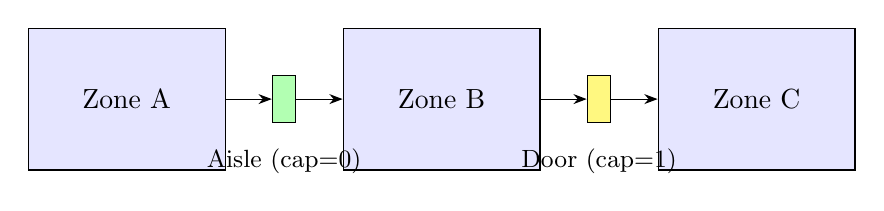
\begin{tikzpicture}[
    zone/.style={rectangle, draw, minimum width=2.5cm, minimum height=1.8cm, fill=blue!10},
    opening/.style={rectangle, draw, minimum width=0.3cm, minimum height=0.6cm}
]
    \node[zone] (z1) at (0,0) {Zone A};
    \node[zone] (z2) at (4,0) {Zone B};
    \node[zone] (z3) at (8,0) {Zone C};
    
    \node[opening, fill=green!30] (aisle) at (2,0) {};
    \node[opening, fill=yellow!50] (door) at (6,0) {};
    
    \draw[-{Stealth}] (z1.east) -- (aisle.west);
    \draw[-{Stealth}] (aisle.east) -- (z2.west);
    \draw[-{Stealth}] (z2.east) -- (door.west);
    \draw[-{Stealth}] (door.east) -- (z3.west);
    
    \node[below=0.2cm of aisle] {\small Aisle (cap=0)};
    \node[below=0.2cm of door] {\small Door (cap=1)};
\end{tikzpicture}
\caption{Aisle and door as opening instances with different capacity}
\end{figure}

%==============================================================================
\section{CAD Import Strategy}
%==============================================================================

\subsection{Priority Order}

\begin{enumerate}
    \item \textbf{DXF (Priority 1)}: Floor plans, walls, equipment outlines. Libraries: \texttt{netDxf}, \texttt{IxMilia.Dxf}. Weekend project.
    
    \item \textbf{IFC (Priority 2)}: If users have BIM models. Semantic building data. Library: \texttt{xBIM}. One week.
    
    \item \textbf{3D Visualization Only (Priority 3)}: Import STEP/glTF as visual proxy. Attach to equipment node. Don't extract geometry from it.
\end{enumerate}

\begin{warning}
\textbf{Never attempt:}
\begin{itemize}
    \item Parse native Solidworks/Inventor files
    \item Auto-extract footprints from STEP assemblies
    \item Build a general CAD kernel
\end{itemize}
\end{warning}

\subsection{DXF Import Flow}

\begin{enumerate}
    \item User selects .dxf file
    \item Show layer list from file
    \item User maps: ``A-WALL'' $\rightarrow$ Infrastructure.Walls
    \item Import with mapping
    \item User reviews, fixes scale (CAD often in mm)
    \item Save to SQLite
\end{enumerate}

%==============================================================================
\section{Unity Integration Specification}
%==============================================================================

\subsection{Unity Responsibilities}

\begin{itemize}
    \item Load facility geometry (extruded from 2D or imported 3D)
    \item Load product geometry (STEP/glTF components)
    \item Read event log from SQLite
    \item Playback: scrub through sim\_time like a video
    \item Animate: parts appear/move, workers at stations, cranes operating
    \item Walkthrough: free camera, VR mode
\end{itemize}

\subsection{Unity Does NOT}

\begin{itemize}
    \item Run simulation logic
    \item Make scheduling decisions
    \item Resolve resource conflicts
    \item Store authoritative state (database is source of truth)
\end{itemize}

\subsection{Playback Implementation}

\begin{lstlisting}[language=C, caption=Unity playback pseudocode]
class SimulationPlayback : MonoBehaviour
{
    float currentSimTime = 0f;
    float playbackSpeed = 1f;
    
    void Update()
    {
        currentSimTime += Time.deltaTime * playbackSpeed;
        
        // Query events in time window
        var events = Database.Query(
            "SELECT * FROM sim_events WHERE sim_time <= ? 
             AND sim_time > ? ORDER BY sim_time",
            currentSimTime, lastSimTime);
        
        foreach (var evt in events)
        {
            ApplyEvent(evt);
        }
    }
    
    void ApplyEvent(SimEvent evt)
    {
        switch (evt.event_type)
        {
            case "Move":
                MoveEntity(evt.entity_id, evt.location_id);
                break;
            case "StartOp":
                StartAnimation(evt.entity_id, evt.data);
                break;
            // etc.
        }
    }
}
\end{lstlisting}

%==============================================================================
\section{Summary of Key Decisions}
%==============================================================================

\begin{enumerate}
    \item \textbf{Architecture}: Three-tier (Layout, Parts, Simulation) with shared SQLite database
    
    \item \textbf{Database}: SQLite as source of truth; PostgreSQL for deployment
    
    \item \textbf{Simulation Engine}: O2DES (don't build custom DES)
    
    \item \textbf{Scheduler}: Use existing engine (don't build)
    
    \item \textbf{3D Visualization}: Unity as separate application reading from database
    
    \item \textbf{2D/3D}: Same architecture, configuration-driven complexity
    
    \item \textbf{Access Constraints}: Model as resources in simulation, not just visual
    
    \item \textbf{Openings}: Doors are instances of openings. Capacity = 0 means unconstrained (no token), capacity $\geq$ 1 means token required. All openings have state machine (Open/Closed/Locked). No 3D geometry needed.
    
    \item \textbf{Temporary Openings}: Existence tied to assembly state for shipbuilding scenarios
    
    \item \textbf{Development}: Parallel tracks (WPF, Unity, Integration)
    
    \item \textbf{Customer}: Shipyard partnership --- real project with real requirements
    
    \item \textbf{Scope}: Solve specific problem first, expand from revenue position
\end{enumerate}

%==============================================================================
\section{Next Actions}
%==============================================================================

\begin{enumerate}
    \item \textbf{This week}: Meet with shipyard contact. Listen. Get sample data.
    
    \item \textbf{Define event schema}: Before building simulation or Unity viewer
    
    \item \textbf{Finish WPF layout editor}: Solidify database schema
    
    \item \textbf{Prototype O2DES integration}: One simple model running
    
    \item \textbf{Prototype Unity viewer}: Load facility, playback one simulation
    
    \item \textbf{Prove round-trip}: Edit in WPF $\rightarrow$ Run simulation $\rightarrow$ View in Unity
\end{enumerate}

\vspace{1cm}
\begin{center}
\textit{Go build it.}
\end{center}

\end{document}
